%
% Introduction
%

\chapterimage{Galileos-telescope-002.pdf} % Chapter heading image

\chapter{Introduction}
\label{chap:Introduction}

\begin{quote}
\begin{flushright}
\emph{If presented with a choice between indifferent alternatives,\\
then one ought to select the simplest one.}\\
Occam’s razor principle 
\end{flushright}
\end{quote}
\bigskip

The pursuit of knowledge typically begins with the identification of a collection of entities we seek to comprehend. The constituents of this collection can be extraordinarily diverse. For instance, mathematicians may focus on mathematical concepts, biologists on living organisms, and engineers on problem-solving machines. Our objective, as researchers, is to gain as much understanding of these entities as possible. This understanding, which allows us to predict the outcomes of our actions, is crucial. For example, we know that applying sufficient heat to a pile of wood will ignite a fire. More challengingly, by observing effects, we can attempt to deduce their causes; a fever may indicate a viral infection. Practical problem-solving hinges on understanding, which entails discerning patterns or regularities enabling us to construct a simplified description or model of the original entities. Such models facilitate our manipulation of these entities for our benefit.

Ideally, we aspire to construct descriptions that allow us to reconstruct the original entities under study. However, for a vast number of entities, particularly abstract ones, this is not achievable. Consequently, we must resort to working with representations - using texts or data that strive to capture as many details of the original entities as feasible. For instance, if we are physicists, an entity's representation could be the outcome of an experiment; for computer scientists, it might be a dataset composed of measurements, and for sociologists, it could be a collection of observed facts. Figure \ref{fig:representationProblem} illustrates this process: while we desire our descriptions to model entities, in reality, they model our artificially constructed representations of those entities.

\begin{figure}[t]
\centering
\begin{tikzpicture}
    \node[draw, ellipse, minimum width=3cm] (entities) at (0,0) {Entities};
    \node[draw, ellipse, minimum width=3cm] (representations) at (5,0) {Representations};
    \node[draw, ellipse, minimum width=3cm] (descriptions) at (10,0) {Descriptions};

    \draw[-{Latex[length=3mm]}] (representations) -- node[above,midway] {encode} (entities);
    \draw[-{Latex[length=3mm]}] (descriptions) -- node[above,midway] {model} (representations);
    \draw[dashed,-{Latex[length=3mm]}] (descriptions) to [bend right=45] node[above,midway] {explain?} (entities);
\end{tikzpicture}
\caption{\label{fig:representationProblem}The Problem of Understanding}
\end{figure}

The fundamental question lies in how effectively our descriptions interpret the original entities through the modelling of the representations that encode those entities. We must take into account various potential sources of error. First, our encoding methodology may not be flawless. In an ideal scenario, if an entity $e$ is ideally represented by the string $r$, in practice, we may be working with another string $r'$ that approximates $r$ but is not identical. This type of error is what we call \emph{miscoding}\index{Miscoding}.

Second, our descriptions may not be perfect. Ideally, a description $d$ should allow us to recreate the string $r'$ (as the string $r$ is typically unknown), but in practice, it generates another string $r''$ that is close to $r'$ but not identical. This second type of error is what we denote as \emph{inaccuracy}\index{Inaccuracy}.

Finally, the third category of errors pertains to the descriptions themselves. Given humans' limited cognitive capabilities, we are interested in the shortest possible description $d$ of $e$ so that we can understand the entity, make predictions, or derive implications. However, our current best-known description $d'$ is likely longer than $d$. We term this third type of error as \emph{surfeit}\index{Surfeit}. 

In conclusion, we amalgamate these three types of errors - miscoding, inaccuracy, and surfeit - into a single metric known as \emph{nescience}\index{Nescience}. This serves as a quantitative measure of our lack of knowledge about an entity.

This chapter provides an accessible introduction to our novel \emph{theory of nescience}, accompanied by a concise review of its principal findings. While avoiding the use of complex mathematics, the chapter maintains a semi-formal description of concepts. To further elucidate the introduced notions, a variety of practical examples are presented throughout.

%
% Section: Entities
%

\section{Entities}

At the heart of our theory is the idea that there exists a non-empty collection of things, or \emph{entities}\index{Entity}, that scientists are trying to understand. This set of entities, which we'll refer to as $\mathcal{E}$, could be composed by anything that has been, is currently being, or can be studied in the future. And, we're assuming that it's possible for science to fully understand and explain at least some of these entities.

It's important to note that $\mathcal{E}$ is not a well defined set, from a mathematical point of view, because the only condition is that it must be nonempty. This broad definition has both upsides and downsides. On one hand, it's a limitation because it means our definition of nescience (how much we don't know) isn't something we can easily calculate or measure, so we have to estimate it in real-world situations. On the other hand, it's an advantage because it means the new ideas and methods we're introducing in this book aren't just limited to solving specific problems in science - they can be used in all kinds of different fields.

In the theory of nescience, we don't allow universal sets - essentially, we can't posit the existence of a set $\mathcal{E}$ that encompasses everything. The complication with universal sets is their violation of Cantor's theorem\index{Cantor's theorem}, as explained in Section \ref{sec:descriptions_entities}. According to Cantor's theorem, the power set $\mathcal{P}(\mathcal{E})$ comprised of all possible subsets of $\mathcal{E}$ has more elements than $\mathcal{E}$ itself, contradicting the premise that $\mathcal{E}$ encapsulates everything. Therefore, in the theory of nescience, $\mathcal{E}$ must represent the set of "something". 

Furthermore, not all conceivable sets are permitted. An instance of this is Russell's paradox\index{Russell's paradox}, which postulates the set $\mathcal{E}$ to consist of all sets that are not members of themselves. The paradox surfaces when we try to determine whether $\mathcal{E}$ itself is a member of itself or not (as explained in Section \ref{sec:descriptions_entities}). Thus, we require each set $\mathcal{E}$ to be confined to a specific type of elements, precluding them from becoming members of themselves.

Typically, the set $\mathcal{E}$ corresponds to a distinct field of knowledge, with its constituent elements varying based on how the theory is practically applied. Instances of such sets of entities might include: a collection of mathematical objects (abstract); the Animalia kingdom (living organisms); recognized and unrecognized human needs (abstract); all potential computer programs (strings of symbols), and so forth.

%
% Section: Representations
%

\section{Representations}

In many instances, entities cannot be directly scrutinized through scientific analysis, particularly if they are abstract. Consequently, we have to work with representations of those entities. We designate the collection of strings that encode the entities of $\mathcal{E}$ as $\mathcal{R_\mathcal{E}}$. These strings, referred to as \emph{representations}\index{Representation}, may differ depending on the application of the theory of nescience. In certain scenarios, entities may inherently be string-based (e.g., computer programs), while others might be abstract objects that require encoding into string format (e.g., human needs). It's worth noting that a single entity $e \in \mathcal{E}$ could correspond to more than one valid representation in $\mathcal{R_\mathcal{E}}$. Transforming abstract entities into symbol strings in a manner that fully captures their complexities and intricacies remains a significant, unresolved challenge. As such, the exact composition of the set $\mathcal{R_\mathcal{E}}$ often remains unknown.

Ideally, we would like to establish an encoding function $f:\mathcal{E} \rightarrow \mathcal{R_\mathcal{E}}$ that maps a set of entities $\mathcal{E}$ to the corresponding set of possible representations. However, in practice, defining such a function is challenging because the set $\mathcal{E}$ is not a well defined set, meaning we can't conclusively determine what should or should not be included in this set. For instance, it will require further research to precisely define what constitutes a human need.

From a theoretical standpoint, the concept of an \emph{oracle Turing machine}\index{Oracle Turing machine} (see Chapter \ref{chap:Computability}) could be employed to tackle this issue. A Turing machine\index{Turing machine} is essentially a mathematical model of computation, whereas an oracle Turing machine can be likened to a computer model with internet access. We could presume that this computer could query a hypothetical external service, situated remotely, to verify whether a specific string $r$ encodes \emph{any} entity of $\mathcal{E}$. Notably, we cannot ask the oracle if the string $r$ is a valid representation of the specific entity $e$ we are interested in, as this would necessitate providing a valid string representation of $e$, which is generally unknown. The concept of the oracle machine, however, allows us to define a function from the collection of finite binary strings to the set of entities $f:\mathcal{B}^\ast \rightarrow \mathcal{E}$.

From a practical perspective, we typically approximate the set $\mathcal{R}_\mathcal{E}$ with another set $\hat{\mathcal{R}}_\mathcal{E} \subseteq \mathcal{B}^\ast$ of strings, which we consider to be adequate representations of the entities of $\mathcal{E}$. In scientific practice, these representations have traditionally taken the form of illustrations or images (e.g., in biology), collections of factual data (e.g., in sociology), or experimental results (e.g., in physics). With recent significant advancements in the capability of computers to gather and store data, a novel and potent method for encoding entities has emerged: using vast data sets as representations. It's essential to note that in the encoding process, our objective is not to find the shortest possible representation of the entities but to seek out high-quality representations.

It's crucial to acknowledge that in numerous practical scenarios, the chosen representations of abstract entities may not fully encapsulate all nuances of the original objects. This means we are grappling with oversimplified abstractions of reality, which could potentially curtail our capacity to make sweeping assertions about nature (see Chapter \ref{chap:Miscoding}).

\begin{example}
\label{ex:animals_DNA}
If we're studying animals (the set $\mathcal{E}$), we could use a binary encoding of their DNA (the set $\mathcal{R_\mathcal{E}}$) as representations. While our current technology doesn't allow us to bring a creature to life solely from its DNA, theoretically, it could be feasible. However, DNA alone doesn't fully replicate the original animal, as it doesn't include life experiences. For instance, how would we represent a cat that only has three legs due to an accident? That detail is not recorded in its DNA. If our goal is to study the traits of certain species, working with the DNA of a representative sample of individuals within each species would be adequate. However, if we're studying specific individuals within a species, we would also need a way to encode each animal's history or the details not encapsulated by the DNA.
\end{example}


\begin{figure}[t]
\centering

\begin{tikzpicture}
  % Oval 1
  \node[draw, ellipse, minimum width=3cm, minimum height=6cm, label=below left:{$\mathcal{E}$}] (oval1) at (-2,0) {};

  % Oval 2
  \node[draw, fill=gray!20, ellipse, minimum width=2cm, minimum height=3cm] (oval2) at (-2,1) {};

  % Small circles inside Oval 2
  \node[draw, fill=black, circle, inner sep=0.05cm, label=below:{$e_1$}] (circle1) at (-2, 1.5) {};
  \node[draw, fill=black, circle, inner sep=0.05cm, label=below:{$e_2$}] (circle2) at (-2, 0.5) {};

  % Small circle inside Oval 1
  \node[draw, fill=black, circle, inner sep=0.05cm, label=below:{$e_3$}] (circle3) at (-2,-1) {};

  % Question mark inside Oval 1
  \node[draw, fill=black, circle, inner sep=0.05cm, label=below:{?}] (question) at (-2,-2) {};

  % Vertical Line
  \draw[thick] (0,-3) -- (0,3);
  \node at (0,-3.5) {oracle};

  % Oval 4
  \node[draw, fill=gray!20, ellipse, minimum width=2cm, minimum height=4cm, label=above right:{$\mathcal{R}_{\mathcal{E}}$}] (oval4) at (2,1) {};

  % Small circles inside Oval 4
  \node[draw, fill=black, circle, inner sep=0.05cm, label=below:{$r_1$}] (circle5) at (2,1.5) {};
  \node[draw, fill=black, circle, inner sep=0.05cm, label=below:{$r_2$}] (circle6) at (2,0.5) {};

  % Oval 3
  \node[draw, ellipse, minimum width=2cm, minimum height=4cm, label=below right:{$\hat{\mathcal{R}}_\mathcal{E}$}] (oval3) at (2,-1) {};

  % Small circle inside Oval 3
  \node[draw, fill=black, circle, inner sep=0.05cm, label=below:{$r_3$}] (circle4) at (2,-2) {};

  % Curved arrows
  \draw[->] (circle5) to[bend right=40] (circle1);
  \draw[->] (circle6) to[bend right=40] (circle2);
  \draw[->] (circle4) to[bend left=40] (question);
\end{tikzpicture}

\caption{\label{fig:entities_topics}Entities and Representations.}
\end{figure}

Working with string representations (the set $\mathcal{R}_\mathcal{E}$) can lead to certain entities not being encoded by any representation (see the gray areas in Figure \ref{fig:entities_topics}, specifically, entity $e_3$ lacks an encoding). For instance, if our set of entities is the set of real numbers, some numbers lack a representation, since we don't allow infinite strings as representations. Intuitively, this suggests that in many knowledge domains, the quantity of problems may exceed the number of solutions. Using approximations of representations (the set $\hat{\mathcal{R}}_\mathcal{E}$) can also lead to some representations encoding incorrect entities (as in the case of representation $r_3$ in Figure \ref{fig:entities_topics}). This is due to our incomplete knowledge possibly leading us to utilize incorrect representations for the entities of $\mathcal{E}$. Another issue with incomplete knowledge is the possibility of 'unknown unknowns'\index{Unknown unknown} - entities whose existence we're unaware of. For instance, representation $r_1$ in Figure \ref{fig:entities_topics} is not part of the set $\hat{\mathcal{R}}_\mathcal{E}$ and is therefore overlooked by researchers despite its representation of a valid entity $e_1$. Our objective includes exploring a procedure to uncover new, previously unknown, research entities from the set $\mathcal{R}_\mathcal{E}$ (refer to Section \ref{sec:intro_research_topics} and Chapter \ref{chap:Interesting-Research-Questions}).

A \emph{research area}\index{Research area} $A$ is a subset of topics, in other words, $A \subset \mathcal{R}_\mathcal{E}$. In a practical context, areas prove valuable when their included topics share a common attribute. Our interest may lie in investigating our knowledge gaps about a particular area. For instance, if the set of topics is "animals", areas could include "invertebrates", "mammals", "birds", "amphibians", "reptiles", and "fish". To gauge our lack of knowledge about an area, we first need to describe the topics encompassed by it. However, as our understanding of the topics constituting an area is generally limited, we can only provide partial descriptions. Furthermore, as our comprehension of a research area evolves, the quantity of topics included in its known subset adjusts accordingly. As a result, we can only examine the properties of areas relative to our present knowledge.

\begin{example}
Should our topic set revolve around "astronomy," a conceivable research area might be "habitable planets," a category wherein we have knowledge of only a few currently. A model for this area could be a description compiled from our existing knowledge of these habitable planets.
\end{example}

%
% Section: Descriptions
%

\section{Descriptions}

Upon identifying the set $\mathcal{R}$ of potential representations, our next task is to devise an appropriate method to describe them. In other words, we need to form theories or models that reflect our understanding of the workings of the world. Our human cognitive abilities are, by nature, limited. Therefore, we often depend on simplified models of nature to interpret observed phenomena and predict the outcomes of our actions.

Defining a valid description for an entity presents a challenging, as yet unresolved, issue. Take for example, the Berry paradox\index{Berry paradox}, which suggests the description, "the smallest positive integer not definable in less than twelve words". This statement itself becomes paradoxical as it essentially describes the number in only eleven words. To sidestep such paradoxes, the theory of nescience necessitates that a description for an entity should be a finite symbol string from which we can effectively and completely reconstruct one of the possible representations of the original entity. By "effectively reconstruct", we mean that our models should be computer programs that print the selected representation upon execution. From the era of Newton, science has focused on mathematical models, essentially pursuing a function set that thoroughly describes natural objects and their interrelations. The theory of nescience extends this concept, mandating that such models should be computable.

Descriptions\index{Description} are typically divided into two components: a Turing machine\index{Turing machine} $TM$ (a computer program) that encapsulates all the regularities found in the entity's representation (the compressible part), and an input string $a$ that contains a literal description of the remaining elements (the non-compressible part). Formally speaking, a description for a representation $r \in \mathcal{R}$ is a string $\langle TM, a \rangle$ where $TM(a) = r$. This dualistic nature of descriptions parallels traditional distinctions such as theories and assumptions, theories and initial conditions, problems and specific problem instances, species and individuals, and so on. For instance, a description might consist of a system-modeling set of differential equations (the compressible part), accompanied by a compilation of initial conditions (the non-compressible part). The precise interpretation of the pair $\langle TM, a \rangle$ relies on the specific characteristics of the entity set to which the theory is applied.

\begin{figure}[t]
\centering
\begin{tikzpicture}

    % Draw ovals
    \node[draw,ellipse,minimum width=2.2cm,minimum height=3cm] (entityOval) at (0,0) {};
    \node[draw,ellipse,minimum width=2.2cm,minimum height=3cm] (representationOval) at (3.5,0) {};
    \node[draw,ellipse,minimum width=2.2cm,minimum height=3cm] (descriptionOval) at (7,0) {};
    
    % Draw circle nodes
    \node[fill=black,circle,label={[font=\footnotesize]below:Entity}] (entity) at (entityOval) {};
    \node[fill=black,circle,label={[font=\footnotesize]below:Representation}] (representation) at (representationOval) {};
    \node[fill=black,circle,label={[font=\footnotesize]below:Description}] (description) at (descriptionOval) {};
    
    % Draw arrows
    \draw[-{Latex[length=3mm]},>=stealth,thick,bend right] (representation.north) to node[above]{encode} (entity.north);
    \draw[-{Latex[length=3mm]},>=stealth,thick,bend right] (description.north) to node[above]{model} (representation.north);

\end{tikzpicture}
\caption{\label{fig:entities_topics_models}Entities, representations and descriptions.}
\end{figure}

Figure \ref{fig:entities_topics_models} visually illustrates the relationship between entities, representations, and descriptions. the set of all potential descriptions is signified by $\mathcal{D}$. Not all possible strings qualify as descriptions, as we insist that descriptions must be rooted in Turing machines, and not all possible descriptions outline valid representations.

\begin{example}
To offer an intuitive perspective, consider studying the macroscopic physical aspects of our world. The set of potential descriptions would incorporate elements such as Aristotelian physics, Cartesian physics, Newtonian physics, Einstein's theory of general relativity, and superstring theory, among others. At present, the best description would be Einstein's theory of general relativity, as the superstring theory is yet to be experimentally verified.
\end{example}

A representation $r \in \mathcal{R}$ can have several descriptions, and hence, the objective of science is to discover the shortest possible description, represented by $d^\star$, that enables us to thoroughly reconstruct the representation $r$. Unfortunately, no method or algorithm exists that, when given a string, returns the most concise computer program that outputs that string (refer to the incomputability result of Kolmogorov complexity in Chapter \ref{chap:Algorithmic_Information}). In particular, no method exists that, when provided with a representation, discerns the shortest possible description. Consequently, science presents a non-computable problem, necessitating the compilation of heuristics that approximate the optimal solution. This compilation of heuristics is what we call a \emph{scientific method}\index{Scientific method}.

The theory of nescience concentrates on comprehending and quantitatively assessing the possible errors in the ideal process depicted in Figure \ref{fig:entities_topics_models}. In Sections \ref{sec:ch1_miscoding}, \ref{sec:introduction:inaccuracy}, and \ref{sec:ch1_surfeit}, we propose a series of metrics to measure each potential source of error. In Section \ref{sec:ch1_nescience}, we explore how to merge all these concepts into a single quantity, called \emph{nescience}. This new nescience metric allows us to quantitatively determine the extent of our ignorance about a research entity.

%
% Section: Miscoding
%

\section{Miscoding}
\label{sec:ch1_miscoding}

As we have seen, for the majority of the scientific disciplines, the set $\mathcal{E}$ of entities under consideration could be composed by abstract elements, or other kind of objects that are not easily represented as a string of symbols. Also, it might happen that our current understanding of the elements of $\mathcal{E}$ is limited, and so, we can not properly encode them. In those cases we have to work with approximate representations instead of the valid representations. We are interested in knowing the error introduced due to the use of these incorrect representations.

\begin{figure}[h]
\centering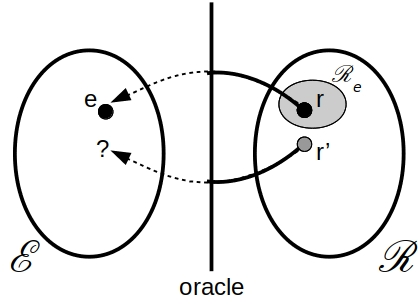
\includegraphics[scale=0.5]{miscoding}
\caption{\label{fig:miscoding}Miscoding of topics.}
\end{figure}

We propose to quantify the \emph{miscoding}\index{Miscoding} of an incorrect representation $r'$ as the length of the shortest computer program that can print the correct representation $r$ having as input $r'$, denoted by $K(r|r')$. See Figure \ref{fig:miscoding}, where $\mathcal{R}_e$ denotes the set of strings that correctly represent the entity $e$. Intuitively, miscoding measures the effort (measured as the length of a program, not as the time it takes to that program to do its work) required to fix the incorrect representation. For example, if our representation contains some errors, the program should be able to identify and correct those errors; or if our representation is missing some critical information required to fully encode the entity, the program will contain, hard-wired, that missing information.

However this approach is not sufficient to fully capture our intuitive notion of miscoding. The problem arises when our represenation $r'$ contains additional information that is not needed to encode the entity $e$. In this case, it might happen that our descriptions include elements modeling those unnecessary symbols, making them artificially long. For example, in a experiment we could be measuring features that do not influence at all the result of the experiment, and given our limited understanding of the original entity, our current description could include those features as predictors\footnote{\color{red} TODO: This example is confusing, since the experiment describes a cause-effect situation, and our machine learning algorithm could identify non-relevant features authomatically. Use a different example.}. In order to avoid this problem, we have to compute also the length of the shortest computer program that can print the incorrect description $r'$ having as input the correct one $r$, that is, $K(r'|r)$. Then, miscoding could be defined as the maximum of these two lengths $\max\{ K(r \mid r'), K(r' \mid r)\}$.

Unfortunately, this last definition still presents some practical problems. Most of the entities have multiple valid representations. Maybe $r'$ is far from a representation $r_1$, but it is closer to a second one $r_2$. It would be unfair to say that a description $d$ that perfectly model $r_2$ is a bad descriptions because it does not model $r_1$, since both, $r_1$ and $r_2$ represent the same entity $e$. A possible solution to this problem would be to look at $\min_{r \in \mathcal{R}_e} \{ \max\{ K(r \mid r'), K(r' \mid r)\} \}$.

\begin{example}
\label{ex:leibnez-wallis}
Let $e$ be the abstract entity called "Pi constant", that is, the ratio of a circle's circumference to its diameter; let $r$ be the Wallis' product\index{Wallis' product} $2 (\frac{2}{1} \cdot \frac{2}{3} \cdot \frac{4}{3} \cdot \frac{4}{5} \cdot \frac{6}{5} \cdot \ldots)$, one of the valid representations of $e$; and let $d$ be the description $\sum_{n=0}^\infty \frac{(-1)^n}{2n+1}$. It would be unfair to affirm that $d$ is a terribly bad description for the entity $e$ because it does not print $r$. In fact, $d$ produces the Leibniz's series\index{Leibniz's series} $4 (1 - \frac{1}{3} + \frac{1}{5} - \frac{1}{7} + \ldots)$ that it is also a valid representation of Pi. Leibniz's series should not be classified as a miscoded representation of Pi, even in the hypothetical case that it were unknown by mathematicians.
\end{example}

As example \ref{ex:leibnez-wallis} pointed it out, one of the most difficult problems with the definition of miscoding is that the set $\mathcal{R}_e$ of valid representations for the entity $e$ is, in general, not known. From a theoretical point of view we could resort again to the oracle Turing machine\index{Oracle Turing machine} to address this problem. However, as we have seen, we cannot ask the oracle if the string $r$ is a valid representation of the entity $e$ in which we are interested (the set $\mathcal{R}_e$), since that would require to provide a valid representation of $e$ as a string of symbols, something that, in general, cannot be done. The only thing we can do is to ask the oracle how far the string $r$ is from being a valid representation of any entity from the set of entities $\mathcal{R}_\mathcal{E}$.

Taking into account all the above considerations, we define the miscoding of a representation $r$, denoted by $\mu(r)$, as:
\[
\mu(r) = \overset{o}{ \underset{r_e \in \mathcal{R}_\mathcal{E}} \min} \frac{ \max\{ K(r_e \mid r), K(r \mid r_e) \} } { \max\{ K(r_e), K(r) \} }
\]
where $\overset{o} \min$ means that the minimum function has to be computed by an oracle. Note that in the definition we have introduced the normalization factor $K(r_e)$, that is, the length of the shortest program that can print $r_e$, because we are interested in comparing the miscoding of multiple, possibly unrelated, representations.

Since miscoding does not take as argument the original entity $e$, it may be the case that what we are representing is not what we were expecting. That is, with our representations and descriptions we might be studying a different entity. This is something that happens quite often in the practice of scientific research. 

\begin{example}
At the end of the eighteenth century, the chemist Joseph Priestley thought he was studying the nonexistent entity called "phlogiston"\index{Phlogiston}, a fire-like element that was supposed to be contained within combustible bodies and released during combustion. It turned out that he was studying a completely different entity called "oxygen".
\end{example}

According to the theory of nescience, our task as researchers is not only to find the proper representations of the entities of $\mathcal{E}$, but also to discover how this ideal oracle machine that knows how to properly encode entities works. That is, why our representations constitute good encodings of the entities under study.

%
% Section: Inaccuracy
%

\section{Inaccuracy}
\label{sec:introduction:inaccuracy}

In the previous section we have characterized how much we do not know about an entity $e$ in terms of the miscoding due to using a wrong representation $r'$ instead of a correct one $r$. In this section we are interested in how much we do not know given a description. Ideally we should be working with a description $d$ that allows us to fully reconstruct the representation $r'$ (recall that the representation $r$ might be unknown), but in general this is not the case in practice. Normally we will be working with a description $d'$ that prints out a string $r''$ (remember that we require that descriptions must be computer programs) that it is (hopefully) close to the string $r'$, but not equal. In this case we say that the description $d'$ is an \emph{inaccurate} description of the representation $r'$ (see Figure \ref{fig:inaccuracy:inaccuracy:inaccuracy}).

\begin{figure}[h]
\centering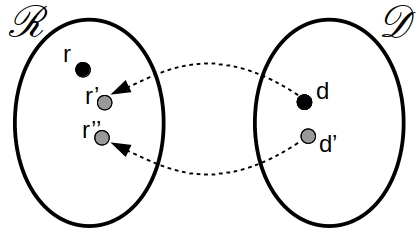
\includegraphics[scale=0.5]{inaccuracy}
\caption{\label{fig:inaccuracy:inaccuracy:inaccuracy}Inaccuracy of a description.}
\end{figure}

If a description is inaccurate for a representation, we would like to have a quantitative measure of how far we are from properly modeling the representation. A natural way to define this measure would be by means of computing the effort required to fix the output of our inaccurate description. In this sense, inaccuracy could be given by the length of the shortest computer program that can print the representation given as input the wrong representation produced by the description. However, as it was the case of miscoding, in order to have a complete picture of the error made with the description $d$ we have to compute also how difficult is to print the inaccurate representation given the good one. It might happen that our description $d$ is modeling things that have nothing to do with the representation $r'$, and simply ignoring those elements is not a solution.

Let $r' \in \mathcal{R}$ be a representation, and $d \in \mathcal{D}$ a description that produces the string $r''$; we define the \emph{inaccuracy}\index{Inaccuracy} of the description $d$ for the representation $r'$, denoted by $\iota(d, r')$, as:
\[
\iota(d, r') = \frac{ \max\{ K(r'' \mid r'), K(r' \mid r'') \} } { \max\{ K(r'), K(r'') \} }
\]
Again, since what we need is the broadest possible interpretation of the concept of inaccuracy, we have to divide by the normalization factor $\max\{ K(r'), K(r'') \}$, so we can compare multiple descriptions for the same representation as well as descriptions for different representations.

We prefer the term \emph{inaccuracy} over the term \emph{error}. Error is given by two components, precision and accuracy. But precision mostly refers to continuous systems, and since we are dealing with discrete strings of symbols, it does not make too much sense to talk about precision in this context.

In practice it is a difficult task to compute the inaccuracy associated with the description of a representation, since, as we have already said, finding the length of the shortest computer program that can print a string is a non-computable problem. If the original entities are texts themselves, the inaccuracy could be approximated using compression algorithms, where the Kolmogorov complexity is approximated with the length of the compressed text using a compressor. If topics are abstract entities, like mathematical concepts, their descriptions could be based on the result of an experiment, and so, the inaccuracy could be based on the error of the model (for example, by means of computing the length of the additional information required to fully describe the results of the experiment given the model). In this sense, our definition of inaccuracy is a generalization of the concept of error, since it can be applied to multiple types of entities, not only to those entities that can be encoded as datasets.

\begin{example}
\label{ex:introduction:inaccuracy:newton}
{\color{red} TODO: Review this example.}
The topic Newton's second law\index{Newton's second law} of motion $F = m a$ could be encoded given the results of an experiment using objects of different masses to which we apply different forces and then we measure the acceleration. The dataset would be composed by the masses, the forces, and the accelerations achieved for each combination of mass and force. However, if we are interested in the acceleration due to gravity, forces and masses cancel out, and so, the only value to measure is acceleration.  Of course, if the result of the experiment is a large collection of measurements, the encoding of the entity would be very long. But, as we said before, with the encodings of entities we are not interested in finding the shortest possible strings, what we are looking for are complete and accurate encodings of topics. For this example we will use the results of an experiment performed by the National Bureau of Standards in Washington D.C. between May 1934 and July 1935. The dataset is composed by 81 measurements, and each value is expressed in centimeters per second squared, for example 980,078. In practice we approximate the quantity $\frac{ K(t \mid m) } {K(t)}$ by $\frac{ C(D \mid M) } {l(D)}$, where $C(D \mid M)$ is the length of the compressed version of the data given the model (using a standard compressor), and $C(D)$ is the length of the compressed data. In order to encode the dataset we require 20 bits per measure (using an uniform code, as it is explained in Chapter \ref{chap:Coding}), and so, to encode the full dataset we require 1,620 bits. If we assume that our model predicts a gravity of $980,000 cm/s^2$ plus a random error that follows a normal distribution (estimated using a maximum likelihood approach), we have that it requires 453 bits to encode the data given the model (see Chapter \ref{chap:Machine-Learning} for more information about how to encode a dataset given a model). We have that the approximated inaccuracy of the model is $\frac{453}{1,620} = 0.27$.
\end{example}

As it was pointed out by Example \ref{ex:introduction:inaccuracy:newton}, when dealing with representations based on experiments, we have to take into account that there is no way, from a logical point of view, to determine which one is the factor that contributes the more to our unknown, a wrong model (inaccuracy) or a wrong experiment (miscoding).


%
% Section: Surfeit
%

\section{Surfeit}
\label{sec:ch1_surfeit}

If it requires a lot of time and effort to explain how something works, we probably do not understand it, and our knowledge must be incomplete. Long descriptions usually contain a lot of things that are not needed, and, in our opinion, one of the main tasks of science should be to reduce as much as possible those unnecessary elements. We relay on descriptions, usually mathematical models, to forecast the future given the past, to understand the relation between causes and effects, and to design machines that solve problems. We have a strong interest in finding the shortest possible models that describe how things work, so they can fit in our limited brain and make our work as scientists and engineers easier\footnote{In a (hopefully) not so long distant future, when all scientific reasoning is performed by computers, having the shortest possible models will no be a priority any more, and it will become a mere scientific curiosity of limited practical value.}.

The theoretical limit of what can be known about a representation, that is, its perfect description $d^\ast$, is given by the shortest possible computer program that allows us to reconstruct the representation. The surfeit of a description $d'$ can be computed by comparing the length of this particular description with the length of the best possible description $d^\ast$ for that representation (see Figure \ref{fig:intro-surfeit}).

\begin{figure}[h]
\centering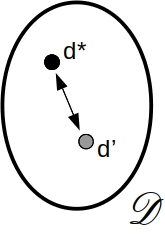
\includegraphics[scale=0.5]{surfeit}
\caption{\label{fig:intro-surfeit}Surfeit of a model.}
\end{figure}

Given an entity $e$, and one of its representations $r$, we define the \emph{surfeit}\index{Surfeit} of the description $d$ for the representation $r$, denoted by $\sigma(d, r)$, by:
\[
\sigma\left(d, r\right) = \frac{l \left(d\right) - K(r)}{l \left(d\right)}
\]

where $l \left(d\right)$ is the length (number of symbols) of the description $d$, and $K(r)$ is the length of the shortest possible description for $r$, that is, $d^\ast$. Since we are interested not only in measuring the surfeit of the description of individual representations, but also in comparing the surfeit of representations for multiple, potentially unrelated, entities, we have to divide the difference $l \left(d\right) - K(r)$ by the normalization factor $l \left(d\right)$. Unfortunately, in general, we do not know the shortest description of a representation, since our knowledge is incomplete, and so, surfeit is a quantity that has to be approximated in practice.

If we were able to come up with a perfect description for a representation, that string of symbols must be incompressible, otherwise it would contain superfluous elements that can be removed, and so, either it is not incompressible or it is not perfect. Given that an incompressible string is a random sequence of symbols (see Section \ref{sec:incompressibility_randomness}), an important consequence of our theory is that perfect knowledge implies randomness\index{Randomness}. The common understanding is that it is not possible to make sense from something that is random, since this is what randomness is all about. However, in the theory of nescience, by random description we mean a model that contains the maximum amount of information in the smallest space possible (it contains no redundant elements). Please mind that the converse does not hold; that is, a random description does not imply perfect knowledge. it might be possible we keep improving a theory until it becomes random, but later on we find a new and shorter theory (probably based on another encoding) that describes the same entity, and this new theory is not random yet.

Randomness effectively imposes a limit to how much we can know about a particular entity. Far from being a handicap, the proper understanding of this absolute epistemological limit is an opportunity to advance in our understanding of open problems. Moreover, since what is limited is the enhancement of our knowledge about already identified research entities, as opposed to the discovery of new ones (new entities are understood to be infinite), we can also apply our understanding of randomness to discover new research entities.

With our definition of surfeit, where longer explanations are worse, we are not suggesting that textbooks should always be as concise as possible. On the contrary, in some situations we expect textbooks to be highly redundant. A concise book is a text that contains a large amount of information in a very reduced space, and so, it is very difficult for humans to assimilate (understand) that information. However, a redundant textbook (like this one) contains the same amount of information but in a lager space, and so, it is easier to grasp it contents. Moreover, in some knowledge areas other than science, redundancy could be desirable. For example, in law, redundancy helps lawyers memorize legal texts, and in music, repetition could be a good thing for harmony, for example in a canon.

The concept of surfeit can be extended to research areas a well, in such a way that we can not only compute the surfeit of a given area as a whole, but also compare the surfeit of multiple, unrelated, areas.

\begin{example}
Based in the concept of "category" of Wikipedia, that it is quite similar to our concept of "research area", we could compute the surfeit of the major scientific areas (see Chapter \ref{chap:Redundancy} for more information about how to compute surfeit in practice). For example, as it is shown in Table \ref{tab:Redundancy_Areas}\footnote{Data from October 2014.}, in general our understanding of Mathematics is higher than our understanding of Computer Science, since the redundancy of Mathematics is 0.351 and the redundancy of Computer Science is 0.443. The concept of redundancy applied to areas largely matches our intuitive notion of which knowledge areas are better understood.
\end{example}

\begin{table*}
\begin{centering}
\begin{tabular}{|c|c|}
\hline 
Kowledge Area & Redundancy \tabularnewline
\hline 
\hline 
Mathematics & $0.351$ \tabularnewline
\hline 
Computer Science & $0.443$ \tabularnewline
\hline 
Chemistry & $0.466$ \tabularnewline
\hline 
Biology & $0.475$ \tabularnewline
\hline 
Psychology & $0.528$ \tabularnewline
\hline 
Epistemology & $0.530$ \tabularnewline
\hline 
Sociology & $0.543$ \tabularnewline
\hline 
\end{tabular}
\par\end{centering}
\caption{\label{tab:Redundancy_Areas}Redundancy of Scientific Areas}
\end{table*}

%
% Section: Nescience
%

\section{Nescience}
\label{sec:ch1_nescience}

Nescience is an old fashioned English word meaning “lack of knowledge or awareness”. In this sense, it seems to mean exactly the same as the word "ignorance", however there is a subtle difference: ignorance refers the lack of knowledge when knowledge is there (we do not know but we could learn, for example, by reading a book), and nescience refers to the lack of knowledge when knowledge is not there (we do not know, and it is not possible to know, since nobody knows). The theory of nescience has been developed with the aim of quantitatively measuring how much we do not know when knowledge is not there, that is, to quantify how much we, as humankind, do not know.

Intuitively, how much we do not know about an entity has to be computed based on the miscoding, inaccuracy and surfeit of a representation and a description, since those metrics summarize all possible types of mistakes we can make. Miscoding because it tell us how well the representation encodes the original entity under study; inaccuracy because it says how well the description models the representation; and surfeit because it tell us how good is the description itself. The best combinations of representations and descriptions are those who present a low miscoding, low inaccuracy and low surfeit. Unfortunately, those quantities are conflicting, in the sense that if we reduce one of them, the others may increase. For example, if we use a more complex description usually the inaccuracy will decrease but the surfeit will increase.

A pair $(d, r)$ composed by a description and a representation is Pareto optimal\index{Pareto optimality} if there does not exist another pair $(d', r')$ such that decreases at least one of the components of nescience, that is miscoding, inaccuracy and surfeit, without increasing another component. We are interested in a local version of the concept of Pareto optimality, since it might happen that the description $d'$ is so far from the description $d$ that it does not represent anymore the entity $e$ encoded by $r$ (given the insight of the oracle).

Pareto optimality allow us to find a family of candidate pairs $(d, r)$ that provide good explanation of an entity $e$. However, in science we prefer to select a single description as the model of a research entity. In order to select that description we have to provide a utility function\index{utility function} that allow us to classify and order the candidate descriptions. The form of this utility function is something that depends on the area in which the theory of nescience is being applied. For example, in case of entities encoded as datasets (machine learning) a good candidate utility function is the harmonic mean (see Chapter \ref{chap:Machine-Learning}). The \emph{harmonic nescience}\index{Nescience} of the representation $r$ given the description $d$ , denoted by $\nu_H\left(d, r\right)$, is defined as:
\[
\nu_H\left(d, r \right) = \frac{3}{ \mu(r)^{-1} + \iota(d, r)^{-1} + \sigma(d, r)^{-1}} 
\]
In the practice of science, we usually fix $r$ and talk about the nescience of the representation $r$ instead of the original entity $e$. If we have multiple candidate models $d_1, d_2, \ldots, d_n$ for the representation $r$, we say that our \emph{current best description}, denoted by $\hat{d}$, is the description that present the lowest nescience given a representation $r$.

\begin{example}
\label{cha1:ex:Boston}
{\color{red} TODO: Review this example.}
We are interested in understanding which are the factors that affect the price of houses. The encoding of that topic will be given by a dataset corresponding to 506 random samples taken from the suburbs of Boston\index{Boston dataset}. For each sample, 14 attributes have been measured, like for example the average number of rooms per dwelling, the per capita crime rate by town or the accessibility to radial highways. Our models will be based on a decision tree (a collection of nested if-else clauses), showing which are the most relevant factors that affect the price. The problem at hand is to identify the ideal depth of that tree, that is, how many if-else decision we should allow in the model that explain the behavior of prices. In order to do that, we compute the best trees from a depth level of 2 to a depth level of 8. In Table \ref{tab:Nescience_Models} left we have a plot of the mean squared error of the best model at each level, using different subsets for training and testing in order to avoid the overfitting of models. As we can see, the optimal level is 5, since increasing beyond this point means that there will be almost no further gain. In Table \ref{tab:Nescience_Models} right we can see the same study but applying our concept of nescience. In this latter case, we see that the optimal level is 3. That is, beyond that level it might be possible that our error decreases, but the model becomes so complex that it makes interpretation very difficult, and so, our understanding of the topic does not increase\footnote{Please mind that nescience and interpretability are not equivalent concepts, in the sense that we can find models with very low nescience that it are beyond the human capabilities of interpretation.}.
\end{example}

\begin{table*}
\begin{centering}
\begin{tabular}{c c}
\centering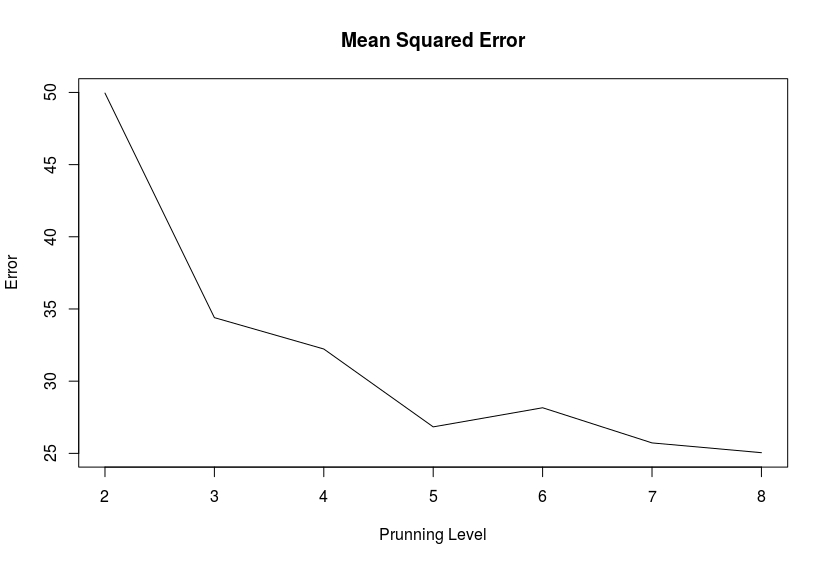
\includegraphics[scale=0.25]{Chapter1_MSE}
&
\centering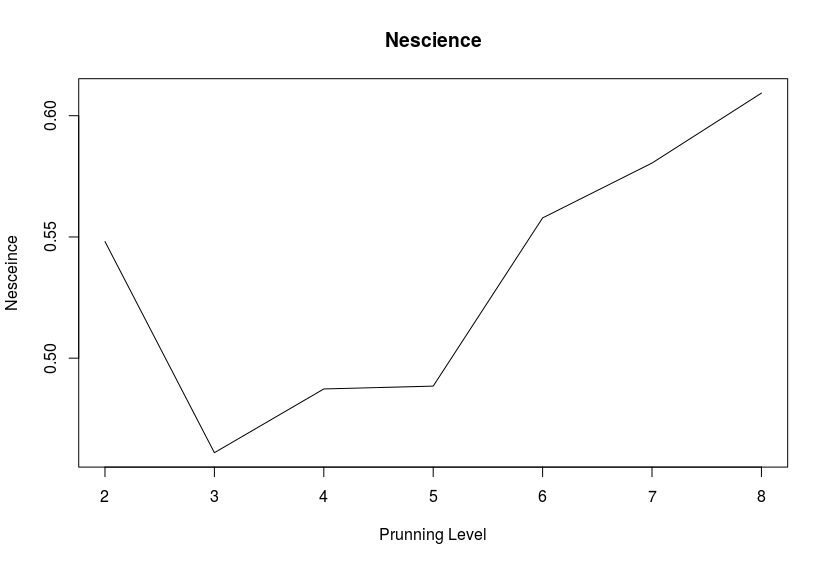
\includegraphics[scale=0.25]{Chapter1_Nescience}
\end{tabular}
\par\end{centering}
\caption{\label{tab:Nescience_Models}RMSE and Nescience of Models}
\end{table*}

We are interested in comparing the nescience, i.e. how much we do not know, of different research entities. For example, mathematicians claim that we do not know almost anything about differential equations, and sociologists claim that we do not know almost anything about the causes of armed conflicts. As it is shown in Example \ref{ex:diffeq_world}, this "we do not know almost anything" is much higher in case of armed conflicts than differential equations.

\begin{example}
\label{ex:diffeq_world}
We can compare how well we understand the "causes of the first world war" with how well we understand the "dynamics of populations", in this particular example, represented by the Lotka–Volterra differential equation\index{Lotka–Volterra differential equation}. In order to compare in practice these research topics we need a description, as complete and accurate as possible, of our current understanding about them. In case of abstract objects, we could use as descriptions the ones contained in reference works, since what we need is an encyclopedic coverage. For this example, we have used the descriptions found in the corresponding pages of the Wikipedia online encyclopedia\footnote{https://en.wikipedia.org/wiki/Causes\_of\_World\_War\_I (retrieved on August 2017)},\footnote{https://en.wikipedia.org/wiki/Lotk-Volterra\_equations (retrieved on August 2017)}. After a pre-processing of the original text, in which Wikimedia tags were removed, the files were compressed with the 7z compression utility (see Chapter \ref{chap:philosophy-science} for a detailed description of this process). Given this approach we have estimated that the redundancy of the causes of the first world war is 0.67, and the redundancy of the dynamics of population is 0.59. Those numbers suggest that we know better how the dynamics of populations work that the causes of this particular armed conflict. Unfortunately, not only is redundancy an approximation of surfeit, but also, in order to fully characterize our unknown we have to take into account the error of both descriptions. Moreover, it might happen that these pages at Wikipedia are not the best current descriptions available for those topics.
\end{example}

When the nescience of a representation $r$ is equal to zero ($\nu(d, r)=0$), we say that we have reached a \emph{perfect knowledge}\index{Perfect knowledge} about an entity. In practice it is not possible to know when we have reached the shortest possible description of the best possible valid representation, that is, when we have found the ultimate theory, since representations require to query the oracle, and descriptions are based on the uncomputable Kolmogorov complexity.

%
% Evolution of Nescience
%

\section{Evolution of Nescience}

In this book we assume that the final objective of science is to discover those descriptions and representations with the lowest possible nescience. The general approach is to produce a series of candidate descriptions and representations over time, each one with a lower nescience than the previous one, until perfect knowledge is reached. New descriptions could be based on novel theories that explain the entity, refinements over already existing ones, reducing the number of assumptions, etc. Nescience can also decrease by means of discovering better representations of the entities under study.

If performed properly, the nescience of an entity should be strictly decreasing as new descriptions and representations appear, since we should not accept a new description or representation as an improvement over the existing ones unless it reduces the nescience. It might happen that a new description presents a higher surfeit, or a higher inaccuracy, but never both things at the same time, since that would imply a higher nescience. Of course, in practice things are not that easy, since our current values of miscoding, inaccuracy and surfeit as just estimations of the real values, and they could be wrong estimations. For a practical point of view, we only require that nescience decrease over time on average.

\begin{example}
The concept of nescience can be applied to measure how well we understand current computer software, like for example operating systems, databases, or productivity applications. The surfeit of the software could be based on the compressibility of the source code, and the inaccuracy on the number of bugs found. In Figure \ref{fig:Chapter1_SQLite} we can see the evolution of the nescience in the latest published versions of the open source database SQLite\footnote{www.sqlite.org}. As we can observe (given the regression line) the nescience of SQLite decreases with time, and so, we can conclude that as new versions appear this application better solves the problem at hand. In Chapter \ref{chap:Software-Engineering} we will see that this is not the case for most of the existing software platforms and applications.
\end{example}

\begin{figure}[h]
\centering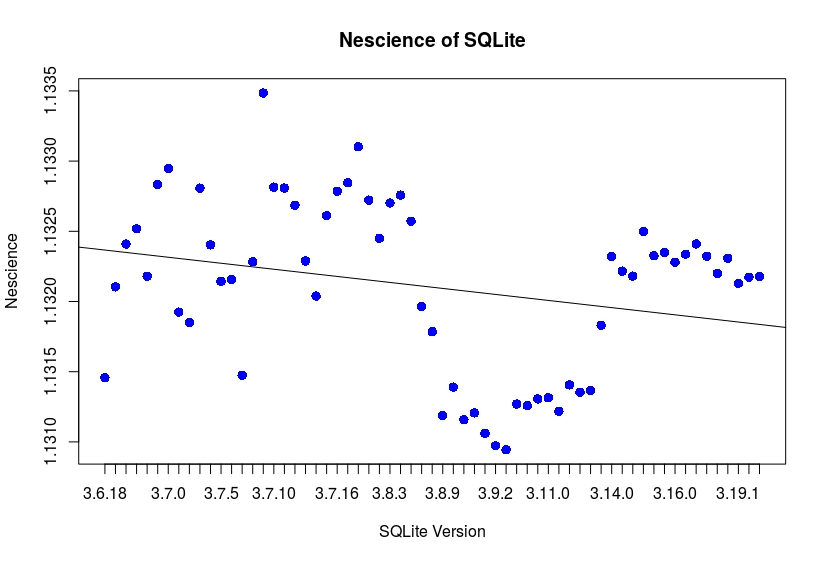
\includegraphics[scale=0.35]{Chapter1_SQLite}
\caption{\label{fig:Chapter1_SQLite}Evolution of Nescience}
\end{figure}

We can use this property of reduction of nescience as a characterization of what constitutes a valid scientific discipline and what is not (what it is called the demarcation problem in philosophy of science). In case of non-scientific theories (pseudosciences and others) nescience does not decrease, on average, when new representations or new descriptions are available. That is, in pseudosciences we do not learn anything new when we do further research.

\begin{example}
A trading robot is a computer program that gets as input real time quotes from the stock markets, or foreign currency exchanges, and based on an algorithm decides how to invest money, in general by means of opening very short-time positions (what it is called intra-day trading). Many of these robots are based on technical indicators, that is, metrics that are derived from current and past prices (like moving averages, or resistance levels) to forecast future prices. It is an open question if it is possible to make any money using those robots, that is, if they have a positive mathematical expectancy sufficiently high to cover brokers commissions. We can study this problem with the aid of the theory of nescience. In order to do that, we have randomly selected 40 trading robots developed over a period of 6 years, and we have tested them (see Section \ref{sec:trading} for more information). In Figure \ref{fig:Chapter1_EA} we can see the evolution of the nescience of these robots along time. As we can observe, nescience does not decrease, in fact it increases.
\end{example}

\begin{figure}[h]
\centering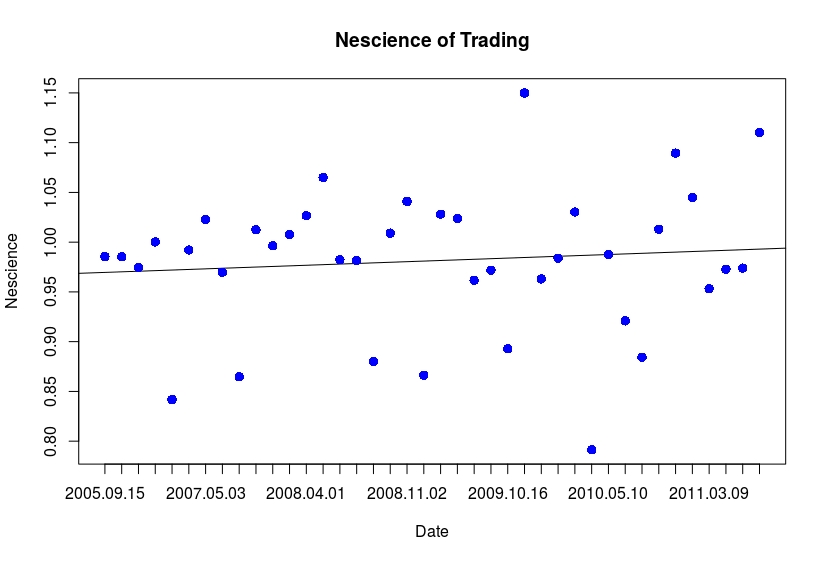
\includegraphics[scale=0.35]{Chapter1_EA}
\caption{\label{fig:Chapter1_EA}Nescience of Forex Trading Robots}
\end{figure}

%
% Section: Other Metrics
%

\section{Other Metrics}

Nescience is a metric that can be used to identify the most interesting topics from the point of view of research. Since nescience is a measure of our ignorance about a topic, the higher the nescience the more opportunities for research. In this section we are going to propose other metrics that can complement nescience in the task of measuring the interest of research topics. These metrics will be helpful, not only for the classification of individual research topics, but also for the development of a methodology for the discovery of potential solutions to open problems (Section \ref{sec:intro_interesting_questions}), and the discovery of new research topics (Section \ref{sec:intro_research_topics}).

One of these new metrics for the classification of research topics is \emph{relevance}. Relevance is a measure of the impact that a topic has on people's life. Intuitively, the higher the relevance of a topic, the higher its potential as a source of interesting problems, since we will be working on problems that affect many people directly. In order to measure the impact of a research topic we have to construct what we call the relevance graph, a figure that describes how people are affected by research topics (see Figure \ref{fig:Relevance-Graph_Intro}).

\begin{figure}[h]
\centering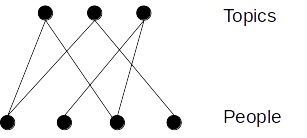
\includegraphics[scale=0.7]{bipartite_graph}
\caption{\label{fig:Relevance-Graph_Intro}Relevance Graph}
\end{figure}

The relevance graph connects all known topics and all possible human beings. A link between a topic and a person means that this person is affected by the topic, not that he is interested in this particular topic. For example, somebody that is trying to find a cure to diabetes will not be connected to the research topic diabetes, however, somebody that actually suffer from diabetes will be. The higher the relevance of a topic, the higher its potential as a source of interesting problems to solve. In this sense, the research topic "how to cure diabetes" is more relevant that the research topic "how far dog fleas can jump", since more people are affected by the former than by the latter. The exact meaning of "\emph{being affected by}" is an abstract concept that has to be approximated in practice. For example, we could claim that the wife of a man that has diabetes is somehow affected by the disease as well. In Part \ref{part:Applications} of this book we will see some examples of how to approximate this abstract quantity.

Given these two metrics, nescience and relevance, we can provide a quantitative measure of the interestingness of a topic as a source of interesting problems, that is, how likely is that the topic can be used as part of a new interesting research project. We define this quantity as a function of the relevance and nescience of the topic (for example, the normalized product of both quantities). Intuitively, a topic is interesting as a source of new problems if it has a large relevance (it has high impact in people's life) and a large nescience (it is not very well understood). In Figure \ref{fig:Interestingness-Questions} is graphically depicted the idea. For example, the Pythagoras' theorem has some relevance, since people life's can be indirectly affected by its implications, but since it is a very well understood theorem (our nescience is very low), it is not a very interesting research topic by itself. The World War I is very relevant, because it had a huge impact on many people's life, and also it is not very well understood topic as we have seen in Example \ref{ex:diffeq_world}. So, according to our definition, it has a huge potential as a source of new interesting research problems.

\begin{figure}[h]
\centering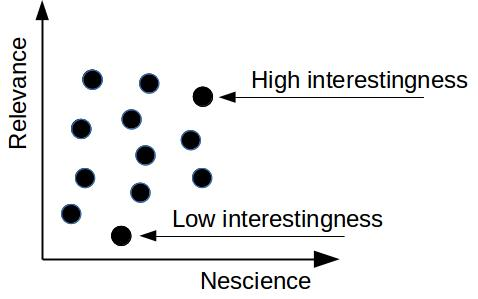
\includegraphics[scale=0.5]{InterestQuestions}
\caption{\label{fig:Interestingness-Questions}Interestingness of Topics}
\end{figure}

\begin{example}
\label{ex:wikipedia-problems}
We can use the collection of Wikipedia articles to identify topics that are interesting as a source of new problems. The starting point of our analysis is the classification contained in the scientific disciplines category of Wikipedia. This category is organized\footnote{Data from November 2014.} into the following main areas: "applied sciences", "behavioral sciences", "cognitive sciences", "formal sciences", "natural sciences", "physical sciences", and "social sciences". In order to evaluate the classification metrics proposed we have used the set of topics corresponding to all pages under any of the subcategories contained in the category "theory of computation" (a subcategory of the category "theoretical computer science", that belongs to the area "formal sciences"). Pages were cleaned up using the same procedure described in Example \ref{ex:diffeq_world}, and the relevance was estimated based on the number of unique visits to each page (please, refer to Chapter \ref{chap:philosophy-science} for more information about this process). Topics that fit our intuitive idea of problem, that is, not very well understood concepts with a high relevance, could include "arithmetical hierarchy" (0.72), "halting problem" (0.65), "floating point" (0.61), "quantum computer" (0.57), and "computable function" (0.55).
\end{example}

The Pythagoras' theorem is not a very interesting research topic by itself, however, it is a very important theorem, since it can be applied to solve many practical problems. A new metric is required to capture this concept of topic that is important because it can be used as a tool to solve other problems. We define the \emph{maturity} of a topic as the inverse of nescience. Intuitively, the more mature a topic is the higher its potential applicability as a tool to solve other open problems, since we know very well how the topic works and how it can be successfully applied. In general, highly immature topics should not be applied to solve open problems, since they could provide wrong answers.

Besides maturity, we also introduce the metric of \emph{applicability} of a topic. Applicability is based on the concept of \emph{applicability graph}. An applicability graph is a directed graph between the research topics (see Figure \ref{fig:ApplicabilityGraph}). An arrow between two topics means that the first topic been successfully applied to explain or solve the second topic. For example, the topic “graph theory” has been applied to the topic “recommendation engines”, since graph theory has been used to solve the problem of which products we should advertise to potential customers on Internet. Given this graph, we define the applicability of a topic as the number of problems to which the topic has been successfully applied. The higher the applicability of a topic, the higher its potential as a tool that can be applied to solve new problems.

\begin{figure}[h]
\centering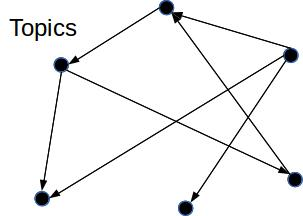
\includegraphics[scale=0.5]{ApplicabilityGraph}
\caption{\label{fig:ApplicabilityGraph}Applicability Graph}
\end{figure}

Finally, we define the concept of interestingness of a topic as a source of interesting tools, that is, how likely is that the topic can be used to solve a new problem, as a function of its maturity and applicability. Intuitively, a topic is interesting as a tool if it has been already applied to many other problems, and it is very well understood topic. For example, the Pythagoras' theorem, although not very relevant as a source of interesting problems, it is very relevant as a source of new applications to other open problems.

\begin{example}
We can use the collection of Wikipedia scientific articles to identify topics with high potential as tools. The procedure used in this example is similar to the one described in Example \ref{ex:wikipedia-problems}, except that the metric applicability has been estimated based in the collection of internal links within Wikipedia itself. The rationale is that if a page is referenced many times by other Wikipedia pages, it is highly likely that it contains useful information. Using this procedure, some examples of topics with high interest as tools in the area of theoretical computer science include "recursion" (0.42), "state space" (0.42), "abstract machine" (0.41), or "ternary numeral system" (0.48).
\end{example}

%
% Section: Interesting questions
%

\section{Interesting Research Questions}
\label{sec:intro_interesting_questions}

In the theory of nescience we distinguish two kinds of unknowns, the \emph{known unknown} and the \emph{unknown unknown}. By known unknown we mean all those already known problems for which we do not know their solutions, for example, nobody knows how to cure diabetes, but we know what diabetes is and we are aware that nobody knows how to cure it. By unknown unknown we mean the collection of unknown problems, that is, all those problems that have not been found yet, like for example the Eldermeyer's disease\footnote{We cannot say anything more about the Eldermeyer's disease, since Dra. Eldermeyer will born next year, and it will take her 34 years more to discover the disease named after her.}. The area composed by the unknown unknown problems is a highly interesting one, since it contains those research topics that will be addressed in the future. One of the main goals of this book is to help scientists discover the topics that lay in this unknown unknown area, since that would bring to the present the research problems of the future (see Section \ref{sec:intro_research_topics}). In this section we focus on how to solve the problems of the known unknown area.

An \emph{interesting question} is a ordered pair of topics $t$ and $p$, where $t$ has a high interestingness as tool, and $p$ has high interestingness as problem. Intuitively, the questions would be something like “can we apply the tool described by topic $t$ to solve the problem described by topic $p$?”. The interestingness of the new questions will be measured by means of a function of the interestingness of $t$ and $p$ themselves. In practice what we have to do is to compute all the possible combinations of tools and questions and select those with higher combined interestingness (see Figure \ref{fig:InterestingQuestions}).

\begin{figure}[h]
\centering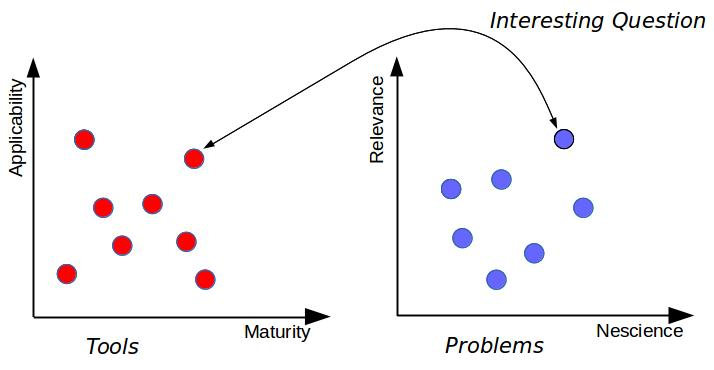
\includegraphics[scale=0.5]{InterestingQuestions}
\caption{\label{fig:InterestingQuestions}Interesting Questions}
\end{figure}

An interesting question is \emph{intradisciplinary} if it combines two topics that are studied in the framework of the same research area (e.g., computer science). An interesting question is \emph{interdisciplinary} if it combines two topics of different research areas (e.g., computer science and philosophy). In principle, the most innovative questions would be interdisciplinary questions, because the probability that somebody has thought about them is lower, since it requires specialists in both research areas working together to come up with that particular question.

\begin{example}
We could combine the topics with high interestingness as tools found in the area of "computer science" with those topics with high interestingness as problems found in the area of "biochemistry" in order to find new interesting interdisciplinary questions. Some examples of the kind of questions we can find with this approach include: “can we use regular expressions to identify DNA genes?” or “can we use a recursive algorithm to characterize proteins tertiary structure?”
\end{example}

Once we have identified an interesting research question, we could use the concept of \emph{conditional model} to see if the tool can help us to understand, or solve, the open problem. A conditional model of a topic $t$ given a perfect model of a second topic $s$ is also a string in the form $\langle TM,a \rangle$, but in this case we require that $TM \left(\langle m_s^\star, a \rangle \right) = t$. That is, the Turin machine $TM$ is able to print $t$ when it has as input both, the incompressible part $a$, and a perfect model $m_s^\star$ for the topic $s$. If the conditional complexity of the open problem given the tool is smaller than its original complexity, then the tool is helpful to solve the problem. The more the tool reduce the length of the conditional model with respect to the original model, the better.

Please note that the methodology presented here is a generic one, in the sense that it can be applied to multiple domains, not only to the discovery of new interesting research questions. The metrics and methods described can be applied to any area where there is a large collection of interrelated describable objects and we are interested in discovering new, previously unconsidered, objects. The exact definition of concepts like relevance graph, applicability graph or maturity will depend on the area in which the methodology is being applied. In Part \ref{part:Applications} of this book, we will describe some examples of other applications, for example, to the identification of new software quality tests.

%
% Section: New Research Entities
%

\section{New Research Entities}
\label{sec:intro_research_topics}

We have mentioned in the previous section the existence of an \emph{unknown unknown} area composed by those problems that not only we do not know how to solve them, but also we are not even aware they exist. We are interested in providing a procedure to discover new research entities located in this important area. A possible approach could be by randomly selecting a binary string and asking to the oracle if that string is close to the representation of a (hopefully unknown) entity. However, given the huge amount of candidate strings, that procedure is not feasible in practice.

In this book we will investigate an alternative approach, based on the combination of already known topics (see Chapter \ref{chap:Interesting-Research-Questions}), what we call \emph{joint topics}. If $r_1, r_2 \in \mathcal{R}$ are two different representations of two different entities, the joint topic of $r_1$ and $r_2$ is the concatenated string $r_1 r_2$ (see Figure \ref{fig:intro_new_topics})\footnote{As we will see in Chapter \ref{cha:Topics-and-Descriptions}, we require $\mathcal{R}$ to be closed under the operation of concatenation of representations, that is, for any two representations $r, s \in \mathcal{R}$ we have that $rs \in \mathcal{R}$.}. For example, if $r_1 \in \mathcal{R}$ is a representation of the entity "maximum entropy", and $r_2 \in \mathcal{R}$ a representation of the entity "probability distribution", the entity represented by the joint topic $r_1 r_2$ would be "maximum entropy probability distribution".

\begin{figure}[h]
\centering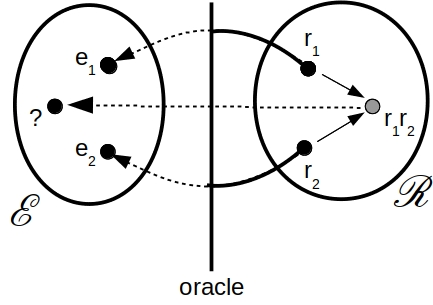
\includegraphics[scale=0.5]{new_topics}
\caption{\label{fig:intro_new_topics}Discovering new research entities.}
\end{figure}

A \emph{new research topic} is a topic that lies in the unknown unknown area. Since the surfeit (resp. inaccuracy) of joining two topics is higher than the superfeit (resp. inaccuracy) of any of them isolated, we can identify new interesting research topics by combining already existing interesting problems (see Figure \ref{fig:NewTopics}). Formally, a new research topic is unordered pair of topics $r_1$ and $r_2$, where both $r_1$ and $r_2$ have a high interestingness as problems. In practice, we have to compute all the possible combinations of those problems with very large interestingness with themselves, and select the ones with the higher potential. The exact meaning of the new topic that results by merging existing problems is something that has to be discovered with further research.

\begin{figure}[h]
\centering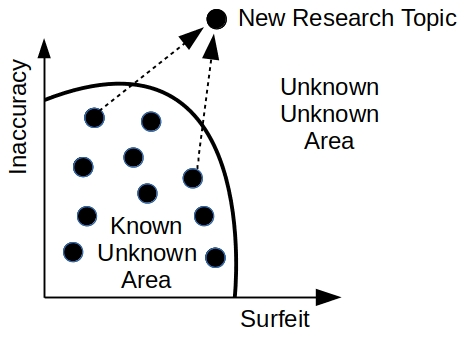
\includegraphics[scale=0.5]{NewTopics}
\caption{\label{fig:NewTopics}New Research Topics}
\end{figure}

\begin{example}
We could combine the most interesting topics of the area of "theoretical computer science" with the most interesting topics of the area "phenomenology" in order to identify the most promising combinations. Fore example, by combining "minimum complexity computer programs" and "self awareness" we obtain that a potential new research topic could be “minimum complexity self-aware computers”; that is, investigating the minimum complexity required for a computer program to have the capacity of being self-aware.
\end{example}

We can extend our method to find new research topics with additional metrics. For example, by means of adding the relevance of topics, we could discover new interesting research topics that are also relevant.

%
% Section: References
%

\section{References and Further Reading}

The idea that perfect descriptions must be random has been already mentioned by other authors (see for example \cite{mosterin2016conceptos}). The gravity dataset used in Example \ref{ex:introduction:inaccuracy:newton} comes from \cite{cressie1982playing}, and a more detailed analysis can be found at \cite{davison1997bootstrap}. The Boston housing dataset referred in Example \ref{cha1:ex:Boston} was published in \cite{harrison1978hedonic} and further discussed in \cite{belsley2005regression}; for more information about decision trees see for example \cite{james2013introduction}. For more information about trading systems and technical indicators see for example \cite{kaufman2013trading}, and how to quantitatively test if a system is profitable to \cite{pardo1992design}. The Locka-Voterra model for population dynamics was originally described in \cite{lotka1920analytical}. How to apply graph analysis to recommendation engines is covered in \cite{cordobes2015empirical}. And finally, if the reader is interested in knowing how far a dog flea can jump, please refer to \cite{cadiergues2000comparison}.

The discipline of epistemology is more oriented to understand what we do know as individuals, meanwhile in this book we are interested in what we know as humankind; moreover, the kind of knowledge addressed by epistemology is not necessarily the scientific knowledge subject of the theory of nescience. Perhaps, the area of epistemology more interesting for our purposes is what the epistemologists call knowing by testimony. A good, and easy to read, introduction to the discipline of epistemology is \cite{nagel2014knowledge}.




